\documentclass[border=0pt]{standalone}
% The shared preamble of every docs diagram (docs/diagrams/<name>.tex).
% dvisvgm's driver first, so patterns and opacity survive into the SVG.
\def\pgfsysdriver{pgfsys-dvisvgm.def}
\usepackage[siunitx,RPvoltages]{circuitikz}
\usepackage{xcolor}
% Latin Modern: outline fonts for every glyph a label uses, µ included.
\usepackage[T1]{fontenc}
\usepackage{lmodern}
\usetikzlibrary{arrows.meta,backgrounds,calc,patterns,positioning}
\tikzset{
  % A white card, so diagrams read in mdBook's dark themes too.
  every picture/.append style={show background rectangle,
    background rectangle/.style={fill=white,inner sep=4pt}},
  % Layout geometry: layers told apart by fill and hatching, never colour alone.
  layer a/.style={draw=black,line width=0.6pt,fill=gray!20},
  layer b/.style={draw=black,line width=0.6pt,fill=gray!45},
  layer c/.style={draw=black,line width=0.6pt,fill=white,postaction={pattern=north east lines}},
  layer d/.style={draw=black,line width=0.6pt,fill=white,postaction={pattern=crosshatch dots}},
  marker/.style={draw=black,dashed,line width=0.6pt},
  % A measured distance and its label.
  dim/.style={{Latex[length=2mm]}-{Latex[length=2mm]},line width=0.5pt},
  dim label/.style={font=\small,fill=white,inner sep=1pt},
  % Where a rule fails: thick, dashed and labelled, not only red.
  violation/.style={draw=red!75!black,line width=1.4pt,dash pattern=on 3pt off 2pt},
  violation label/.style={font=\small\bfseries,text=red!75!black},
  caption/.style={font=\small},
}

\begin{document}
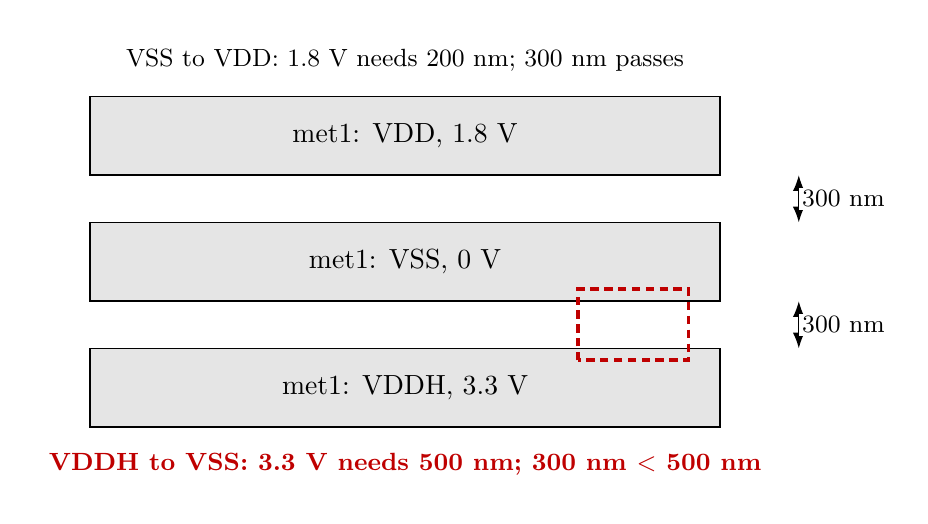
\begin{tikzpicture}
  % Three met1 lines from above, 0.5 um wide, 0.3 um apart (y scaled x4).
  \draw[layer a] (0,0) rectangle (8,1.0) node[pos=0.5]{met1: VDDH, 3.3 V};
  \draw[layer a] (0,1.6) rectangle (8,2.6) node[pos=0.5]{met1: VSS, 0 V};
  \draw[layer a] (0,3.2) rectangle (8,4.2) node[pos=0.5]{met1: VDD, 1.8 V};
  \draw[dim] (9,1.0) -- (9,1.6) node[midway,right,dim label]{300 nm};
  \draw[dim] (9,2.6) -- (9,3.2) node[midway,right,dim label]{300 nm};
  \draw[violation] (6.2,0.85) rectangle (7.6,1.75);
  \node[violation label,anchor=north] at (4,-0.2) {VDDH to VSS: 3.3 V needs 500 nm; 300 nm $<$ 500 nm};
  \node[caption,anchor=south] at (4,4.4) {VSS to VDD: 1.8 V needs 200 nm; 300 nm passes};
\end{tikzpicture}
\end{document}
